% compile with: pdflatex -shell-escape filename.tex
\documentclass[crop,tikz,convert=pdf2svg]{standalone}
\usepackage{pgfplots}
\usetikzlibrary{backgrounds}

\begin{document}

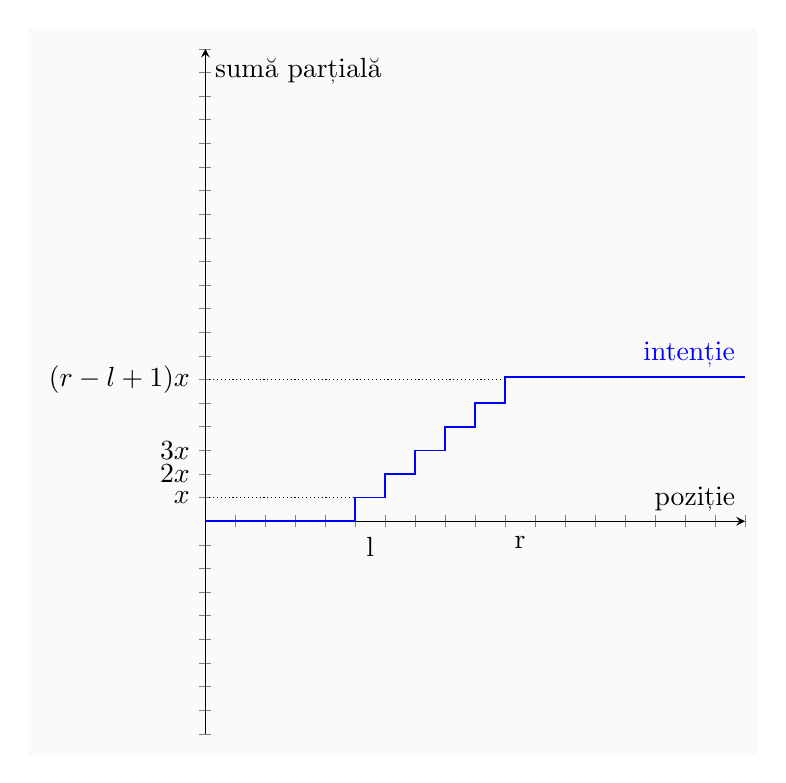
\begin{tikzpicture}[background rectangle/.style={fill=black!02}, show background rectangle]
  \begin{axis}[
      axis lines = middle,
      xlabel=poziție,
      xmin=0,
      xtick distance=1,
      x tick label as interval,
      xticklabels={,,,,,,l,,,,,r},
      y=0.3cm,
      ylabel=sumă parțială,
      ymax=20,
      ymin=-9,
      ytick distance=1,
      %yticklabels={,,$-(l-1)x$,,,,,,,,,$x$,$2x$,$3x$,,,$(r-l+1)x$,,,$lx$,,,,,$rx$},
      yticklabels={,,,,,,,,,,,$x$,$2x$,$3x$,,,$(r-l+1)x$,,,,,,,,},
    ]

    \addplot+[const plot, no marks, semithick]
    coordinates {(0,0) (5,0) (5,1) (6,1) (6,2) (7,2) (7,3) (8,3) (8,4) (9,4) (9,5) (10,5) (10,6.1) (18,6.1)}
    node[pos=1,above left] {intenție};

    % \addplot+[const plot, no marks, semithick]
    % coordinates {(0,0.1) (4.9,0.1) (4.9,9) (6,9) (6,10) (7,10) (7,11) (8,11) (8,12) (9,12) (9,13) (10,13) (10,14) (11,14) (11,0) (18,0)}
    % node[pos=0.57,above right] {$\mathrm{sum}(k) * k$};

    % \addplot+[const plot, no marks, semithick]
    % coordinates {(0,-0.1) (5,-0.1) (5,-8) (11.1,-8) (11.1,6) (18,6)}
    % node[pos=1,below left] {compensare};

    % \addplot+[const plot, no marks, black, densely dotted] coordinates {(0,-8) (5,-8)};
    \addplot+[const plot, no marks, black, densely dotted] coordinates {(0,1) (5,1)};
    \addplot+[const plot, no marks, black, densely dotted] coordinates {(0,6) (10,6)};
    % \addplot+[const plot, no marks, black, densely dotted] coordinates {(0,9) (5,9)};
    % \addplot+[const plot, no marks, black, densely dotted] coordinates {(0,14) (10,14)};
  \end{axis}
\end{tikzpicture}

\end{document}
